\FChapter{Chapter Twelve}{12}

\Lettrine{T}{he} \textsc{promise} of a smooth career, which my first calm introduction to
Thornfield Hall seemed to pledge, was not belied on a longer
acquaintance with the place and its inmates. \Mrs{} Fairfax turned out to
be what she appeared, a placid-tempered, kind-natured woman, of
competent education and average intelligence. My pupil was a lively
child, who had been spoilt and indulged, and therefore was sometimes
wayward; but as she was committed entirely to my care, and no
injudicious interference from any quarter ever thwarted my plans for her
improvement, she soon forgot her little freaks, and became obedient and
teachable. She had no great talents, no marked traits of character, no
peculiar development of feeling or taste which raised her one inch above
the ordinary level of childhood; but neither had she any deficiency or
vice which sunk her below it. She made reasonable progress, entertained
for me a vivacious, though perhaps not very profound, affection; and by
her simplicity, gay prattle, and efforts to please, inspired me, in
return, with a degree of attachment sufficient to make us both content
in each other's society.

This, \foreignlanguage{french}{\emph{par parenthèse}}, will be thought cool language by persons
who entertain solemn doctrines about the angelic nature of children, and
the duty of those charged with their education to conceive for them an
idolatrous devotion: but I am not writing to flatter parental egotism,
to echo cant, or prop up humbug; I am merely telling the truth. I felt
a conscientious solicitude for Adèle's welfare and progress, and a quiet
liking for her little self: just as I cherished towards \Mrs{} Fairfax a
thankfulness for her kindness, and a pleasure in her society
proportionate to the tranquil regard she had for me, and the moderation
of her mind and character.

Anybody may blame me who likes, when I add further, that, now and then,
when I took a walk by myself in the grounds; when I went down to the
gates and looked through them along the road; or when, while Adèle
played with her nurse, and \Mrs{} Fairfax made jellies in the storeroom, I
climbed the three staircases, raised the trap-door of the attic, and
having reached the leads, looked out afar over sequestered field and
hill, and along dim sky-line---that then I longed for a power of vision
which might overpass that limit; which might reach the busy world,
towns, regions full of life I had heard of but never seen---that then I
desired more of practical experience than I possessed; more of
intercourse with my kind, of acquaintance with variety of character,
than was here within my reach. I valued what was good in \Mrs{} Fairfax,
and what was good in Adèle; but I believed in the existence of other and
more vivid kinds of goodness, and what I believed in I wished to behold.

Who blames me? Many, no doubt; and I shall be called discontented. I
could not help it: the restlessness was in my nature; it agitated me to
pain sometimes. Then my sole relief was to walk along the corridor of
the third storey, backwards and forwards, safe in the silence and
solitude of the spot, and allow my mind's eye to dwell on whatever
bright visions rose before it---and, certainly, they were many and
glowing; to let my heart be heaved by the exultant movement, which,
while it swelled it in trouble, expanded it with life; and, best of all,
to open my inward ear to a tale that was never ended---a tale my
imagination created, and narrated continuously; quickened with all of
incident, life, fire, feeling, that I desired and had not in my actual
existence.

It is in vain to say human beings ought to be satisfied with
tranquillity: they must have action; and they will make it if they
cannot find it. Millions are condemned to a stiller doom than mine, and
millions are in silent revolt against their lot. Nobody knows how many
rebellions besides political rebellions ferment in the masses of life
which people earth. Women are supposed to be very calm generally: but
women feel just as men feel; they need exercise for their faculties, and
a field for their efforts, as much as their brothers do; they suffer
from too rigid a restraint, too absolute a stagnation, precisely as men
would suffer; and it is narrow-minded in their more privileged
fellow-creatures to say that they ought to confine themselves to making
puddings and knitting stockings, to playing on the piano and
embroidering bags. It is thoughtless to condemn them, or laugh at them,
if they seek to do more or learn more than custom has pronounced
necessary for their sex.

When thus alone, I not unfrequently heard Grace Poole's laugh: the same
peal, the same low, slow ha! ha! which, when first heard, had thrilled
me: I heard, too, her eccentric murmurs; stranger than her laugh. There
were days when she was quite silent; but there were others when I could
not account for the sounds she made. Sometimes I saw her: she would
come out of her room with a basin, or a plate, or a tray in her hand, go
down to the kitchen and shortly return, generally (oh, romantic reader,
forgive me for telling the plain truth!) bearing a pot of porter. Her
appearance always acted as a damper to the curiosity raised by her oral
oddities: hard-featured and staid, she had no point to which interest
could attach. I made some attempts to draw her into conversation, but
she seemed a person of few words: a monosyllabic reply usually cut short
every effort of that sort.

The other members of the household, viz., John and his wife, Leah the
housemaid, and Sophie the French nurse, were decent people; but in no
respect remarkable; with Sophie I used to talk French, and sometimes I
asked her questions about her native country; but she was not of a
descriptive or narrative turn, and generally gave such vapid and
confused answers as were calculated rather to check than encourage
inquiry.

October, November, December passed away. One afternoon in January, \Mrs{}
Fairfax had begged a holiday for Adèle, because she had a cold; and, as
Adèle seconded the request with an ardour that reminded me how precious
occasional holidays had been to me in my own childhood, I accorded it,
deeming that I did well in showing pliability on the point. It was a
fine, calm day, though very cold; I was tired of sitting still in the
library through a whole long morning: \Mrs{} Fairfax had just written a
letter which was waiting to be posted, so I put on my bonnet and cloak
and volunteered to carry it to Hay; the distance, two miles, would be a
pleasant winter afternoon walk. Having seen Adèle comfortably seated in
her little chair by \Mrs{} Fairfax's parlour fireside, and given her her
best wax doll (which I usually kept enveloped in silver paper in a
drawer) to play with, and a story-book for change of amusement; and
having replied to her \foreignquote{french}{Revenez bientôt, ma bonne amie, ma chère
Mdlle. Jeannette,}\footnote{\enquote{Come back soon, my good friend, my dear Miss Jeannie.}} with a kiss I set out.

The ground was hard, the air was still, my road was lonely; I walked
fast till I got warm, and then I walked slowly to enjoy and analyse the
species of pleasure brooding for me in the hour and situation. It was
three o'clock; the church bell tolled as I passed under the belfry: the
charm of the hour lay in its approaching dimness, in the low-gliding and
pale-beaming sun. I was a mile from Thornfield, in a lane noted for
wild roses in summer, for nuts and blackberries in autumn, and even now
possessing a few coral treasures in hips and haws, but whose best winter
delight lay in its utter solitude and leafless repose. If a breath of
air stirred, it made no sound here; for there was not a holly, not an
evergreen to rustle, and the stripped hawthorn and hazel bushes were as
still as the white, worn stones which causewayed the middle of the
path. Far and wide, on each side, there were only fields, where no
cattle now browsed; and the little brown birds, which stirred
occasionally in the hedge, looked like single russet leaves that had
forgotten to drop.

This lane inclined up-hill all the way to Hay; having reached the
middle, I sat down on a stile which led thence into a field. Gathering
my mantle about me, and sheltering my hands in my muff, I did not feel
the cold, though it froze keenly; as was attested by a sheet of ice
covering the causeway, where a little brooklet, now congealed, had
overflowed after a rapid thaw some days since. From my seat I could
look down on Thornfield: the grey and battlemented hall was the
principal object in the vale below me; its woods and dark rookery rose
against the west. I lingered till the sun went down amongst the trees,
and sank crimson and clear behind them. I then turned eastward.

On the hill-top above me sat the rising moon; pale yet as a cloud, but
brightening momentarily, she looked over Hay, which, half lost in trees,
sent up a blue smoke from its few chimneys: it was yet a mile distant,
but in the absolute hush I could hear plainly its thin murmurs of life. 
My ear, too, felt the flow of currents; in what dales and depths I could
not tell: but there were many hills beyond Hay, and doubtless many becks
threading their passes. That evening calm betrayed alike the tinkle of
the nearest streams, the sough of the most remote.

A rude noise broke on these fine ripplings and whisperings, at once so
far away and so clear: a positive tramp, tramp, a metallic clatter,
which effaced the soft wave-wanderings; as, in a picture, the solid mass
of a crag, or the rough boles of a great oak, drawn in dark and strong
on the foreground, efface the aërial distance of azure hill, sunny
horizon, and blended clouds where tint melts into tint.

The din was on the causeway: a horse was coming; the windings of the
lane yet hid it, but it approached. I was just leaving the stile; yet,
as the path was narrow, I sat still to let it go by. In those days I
was young, and all sorts of fancies bright and dark tenanted my mind:
the memories of nursery stories were there amongst other rubbish; and
when they recurred, maturing youth added to them a vigour and vividness
beyond what childhood could give. As this horse approached, and as I
watched for it to appear through the dusk, I remembered certain of
Bessie's tales, wherein figured a North-of-England spirit called a
\enquote{Gytrash,} which, in the form of horse, mule, or large dog,
haunted solitary ways, and sometimes came upon belated travellers, as
this horse was now coming upon me.

It was very near, but not yet in sight; when, in addition to the tramp,
tramp, I heard a rush under the hedge, and close down by the hazel stems
glided a great dog, whose black and white colour made him a distinct
object against the trees. It was exactly one form of Bessie's
Gytrash---a lion-like creature with long hair and a huge head: it passed
me, however, quietly enough; not staying to look up, with strange
pretercanine eyes, in my face, as I half expected it would. The horse
followed,---a tall steed, and on its back a rider. The man, the human
being, broke the spell at once. Nothing ever rode the Gytrash: it was
always alone; and goblins, to my notions, though they might tenant the
dumb carcasses of beasts, could scarce covet shelter in the commonplace
human form. No Gytrash was this,---only a traveller taking the short
cut to Millcote. He passed, and I went on; a few steps, and I turned: a
sliding sound and an exclamation of \enquote{What the deuce is to do
now?} and a clattering tumble, arrested my attention. Man and horse
were down; they had slipped on the sheet of ice which glazed the
causeway. The dog came bounding back, and seeing his master in a
predicament, and hearing the horse groan, barked till the evening hills
echoed the sound, which was deep in proportion to his magnitude. He
snuffed round the prostrate group, and then he ran up to me; it was all
he could do,---there was no other help at hand to summon. I obeyed him,
and walked down to the traveller, by this time struggling himself free
of his steed. His efforts were so vigorous, I thought he could not be
much hurt; but I asked him the question---

\enquote{Are you injured, sir?}

I think he was swearing, but am not certain; however, he was pronouncing
some formula which prevented him from replying to me directly.

\enquote{Can I do anything?} I asked again.

\enquote{You must just stand on one side,} he answered as he rose, first
to his knees, and then to his feet. I did; whereupon began a heaving,
stamping, clattering process, accompanied by a barking and baying which
removed me effectually some yards' distance; but I would not be driven
quite away till I saw the event. This was finally fortunate; the horse
was re-established, and the dog was silenced with a \enquote{Down,
Pilot!} The traveller now, stooping, felt his foot and leg, as if
trying whether they were sound; apparently something ailed them, for he
halted to the stile whence I had just risen, and sat down.

I was in the mood for being useful, or at least officious, I think, for
I now drew near him again.

\enquote{If you are hurt, and want help, sir, I can fetch some one
either from Thornfield Hall or from Hay.}

\enquote{Thank you: I shall do: I have no broken bones,---only a
sprain;} and again he stood up and tried his foot, but the result
extorted an involuntary \enquote{Ugh!}

Something of daylight still lingered, and the moon was waxing bright: I
could see him plainly. His figure was enveloped in a riding cloak, fur
collared and steel clasped; its details were not apparent, but I traced
the general points of middle height and considerable breadth of chest. 
He had a dark face, with stern features and a heavy brow; his eyes and
gathered eyebrows looked ireful and thwarted just now; he was past
youth, but had not reached middle-age; perhaps he might be thirty-five. 
I felt no fear of him, and but little shyness. Had he been a handsome,
heroic-looking young gentleman, I should not have dared to stand thus
questioning him against his will, and offering my services unasked. I
had hardly ever seen a handsome youth; never in my life spoken to one. 
I had a theoretical reverence and homage for beauty, elegance,
gallantry, fascination; but had I met those qualities incarnate in
masculine shape, I should have known instinctively that they neither had
nor could have sympathy with anything in me, and should have shunned
them as one would fire, lightning, or anything else that is bright but
antipathetic.

If even this stranger had smiled and been good-humoured to me when I
addressed him; if he had put off my offer of assistance gaily and with
thanks, I should have gone on my way and not felt any vocation to renew
inquiries: but the frown, the roughness of the traveller, set me at my
ease: I retained my station when he waved to me to go, and announced---

\enquote{I cannot think of leaving you, sir, at so late an hour, in this
solitary lane, till I see you are fit to mount your horse.}

He looked at me when I said this; he had hardly turned his eyes in my
direction before.

\enquote{I should think you ought to be at home yourself,} said he,
\enquote{if you have a home in this neighbourhood: where do you come
from?}

\enquote{From just below; and I am not at all afraid of being out late
when it is moonlight: I will run over to Hay for you with pleasure, if
you wish it: indeed, I am going there to post a letter.}

\enquote{You live just below---do you mean at that house with the
battlements?} pointing to Thornfield Hall, on which the moon cast a
hoary gleam, bringing it out distinct and pale from the woods that, by
contrast with the western sky, now seemed one mass of shadow.

\enquote{Yes, sir.}

\enquote{Whose house is it?}

\enquote{\Mr{} Rochester's.}

\enquote{Do you know \Mr{} Rochester?}

\enquote{No, I have never seen him.}

\enquote{He is not resident, then?}

\enquote{No.}

\enquote{Can you tell me where he is?}

\enquote{I cannot.}

\enquote{You are not a servant at the hall, of course. You are---} He
stopped, ran his eye over my dress, which, as usual, was quite simple: a
black merino cloak, a black beaver bonnet; neither of them half fine
enough for a lady's-maid. He seemed puzzled to decide what I was; I
helped him.

\enquote{I am the governess.}

\enquote{Ah, the governess!} he repeated; \enquote{deuce take me, if I
had not forgotten! The governess!} and again my raiment underwent
scrutiny. In two minutes he rose from the stile: his face expressed
pain when he tried to move.

\enquote{I cannot commission you to fetch help,} he said; \enquote{but
you may help me a little yourself, if you will be so kind.}

\enquote{Yes, sir.}

\enquote{You have not an umbrella that I can use as a stick?}

\enquote{No.}

\enquote{Try to get hold of my horse's bridle and lead him to me: you
are not afraid?}

I should have been afraid to touch a horse when alone, but when told to
do it, I was disposed to obey. I put down my muff on the stile, and
went up to the tall steed; I endeavoured to catch the bridle, but it was
a spirited thing, and would not let me come near its head; I made effort
on effort, though in vain: meantime, I was mortally afraid of its
trampling fore-feet. The traveller waited and watched for some time,
and at last he laughed.

\begin{figure}
	\begin{sidecaption}{I was mortally afraid of\linebreak its trampling fore-feet.}[p107b]
		\centering
		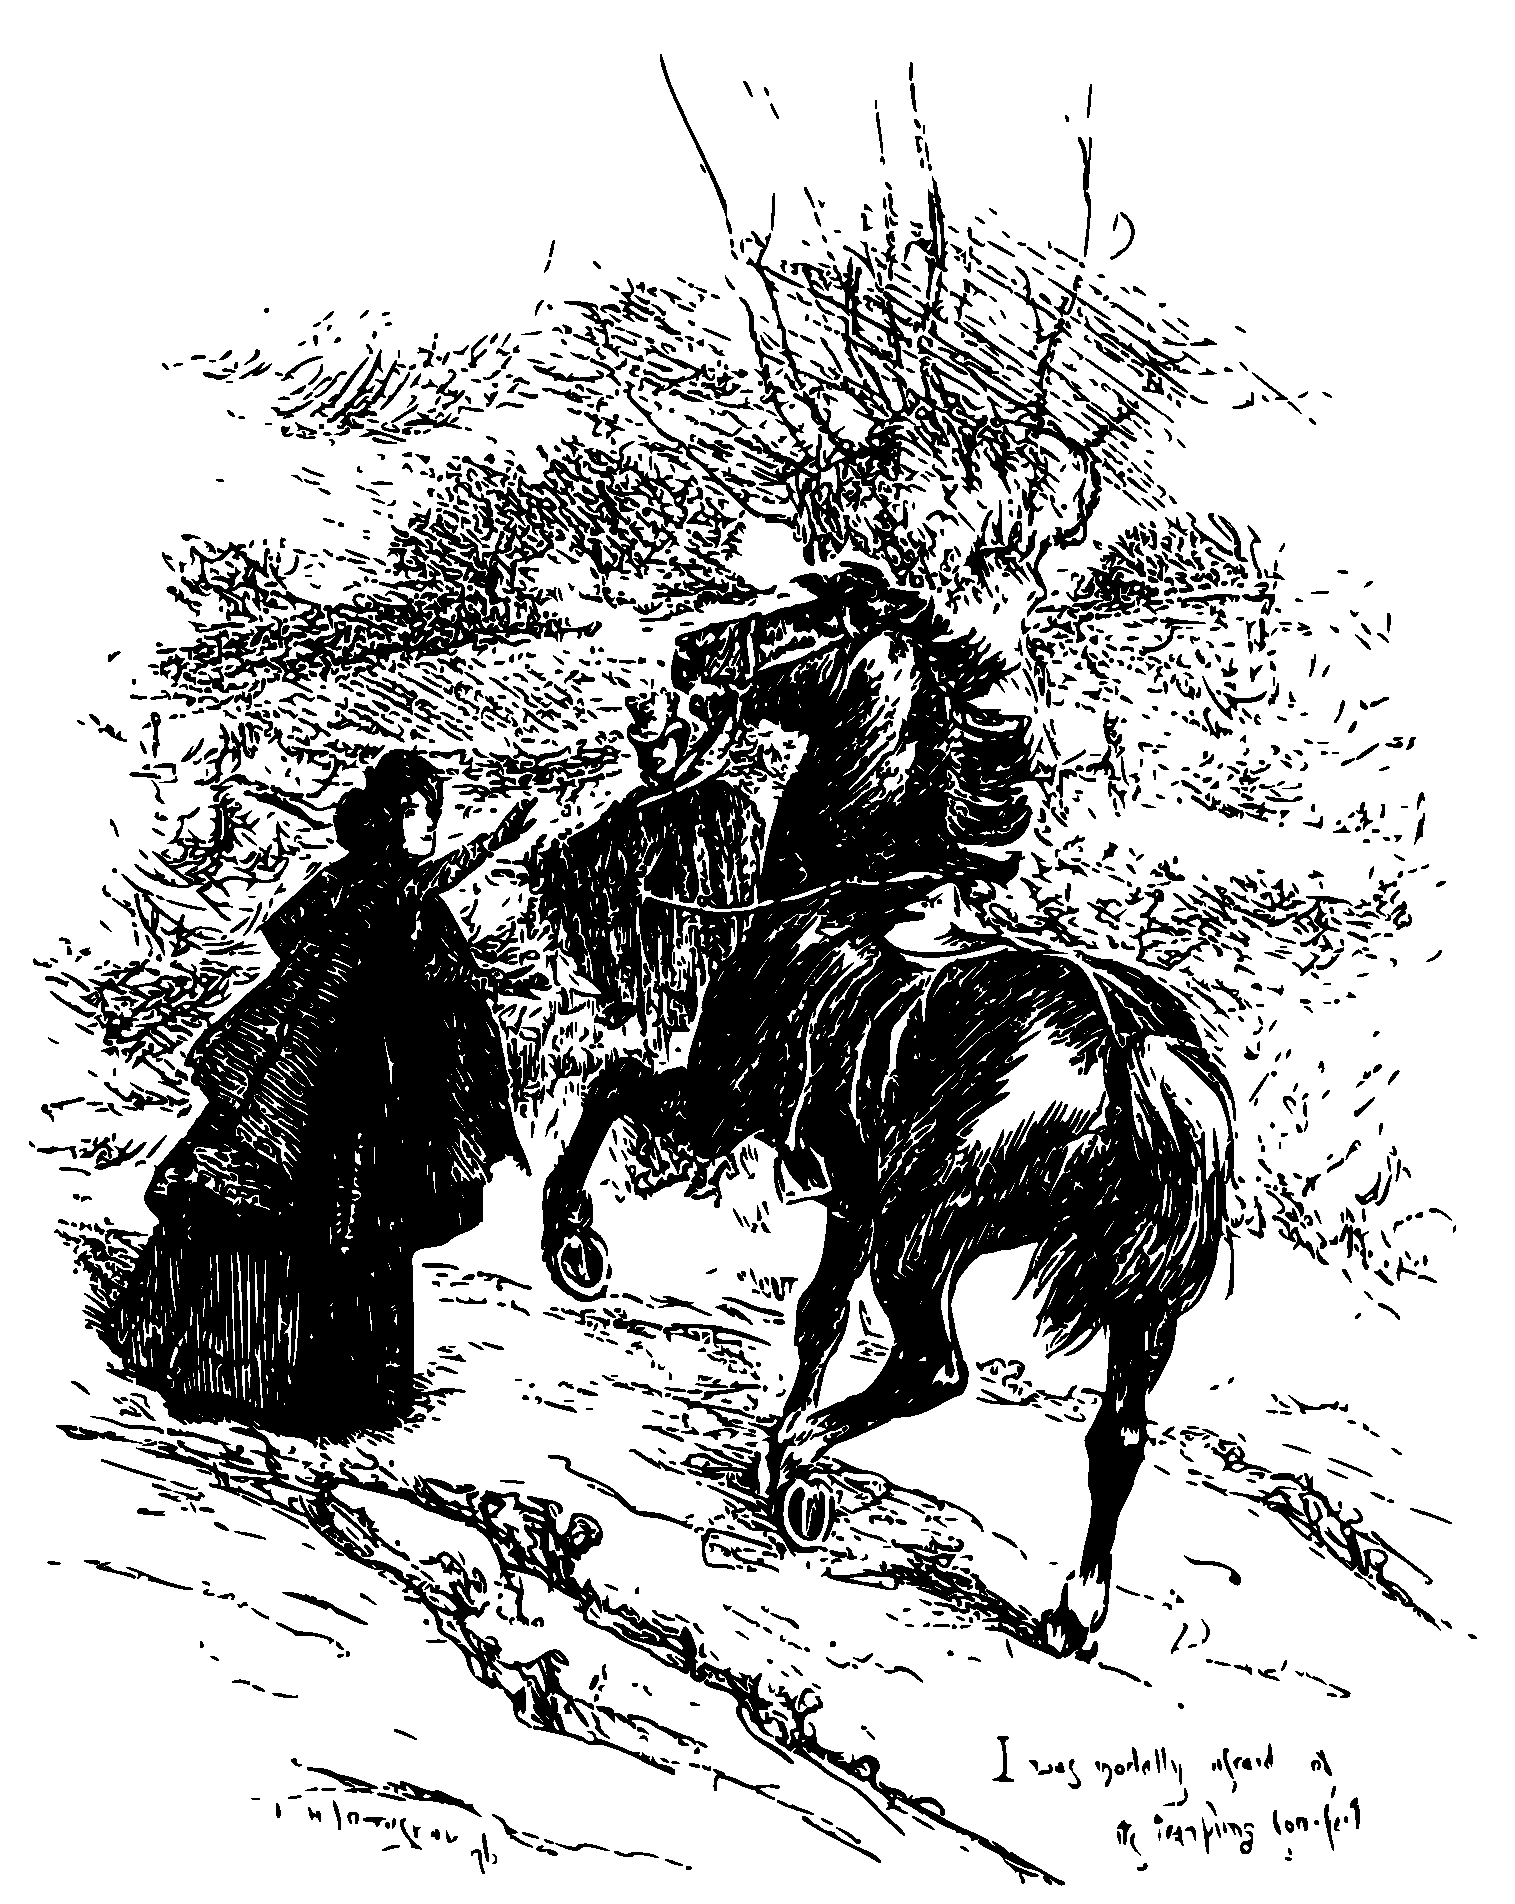
\includegraphics[width=\linewidth]{images/p107b.pdf}
	\end{sidecaption}
\end{figure}

\enquote{I see,} he said, \enquote{the mountain will never be brought to
Mahomet, so all you can do is to aid Mahomet to go to the mountain; I
must beg of you to come here.}

I came. \enquote{Excuse me,} he continued: \enquote{necessity compels
me to make you useful.} He laid a heavy hand on my shoulder, and
leaning on me with some stress, limped to his horse. Having once caught
the bridle, he mastered it directly and sprang to his saddle; grimacing
grimly as he made the effort, for it wrenched his sprain.

\enquote{Now,} said he, releasing his under lip from a hard bite,
\enquote{just hand me my whip; it lies there under the hedge.}

I sought it and found it.

\enquote{Thank you; now make haste with the letter to Hay, and return as
fast as you can.}

A touch of a spurred heel made his horse first start and rear, and then
bound away; the dog rushed in his traces; all three vanished,

\settoversewidth{\versewidth}{'Like heath that, in the wilderness,}
\begin{verse}[\versewidth]
\enquote{Like heath that, in the wilderness,\\*
The wild wind whirls away.}
\end{verse}

I took up my muff and walked on. The incident had occurred and was gone
for me: it \emph{was} an incident of no moment, no romance, no interest
in a sense; yet it marked with change one single hour of a monotonous
life. My help had been needed and claimed; I had given it: I was
pleased to have done something; trivial, transitory though the deed was,
it was yet an active thing, and I was weary of an existence all
passive. The new face, too, was like a new picture introduced to the
gallery of memory; and it was dissimilar to all the others hanging
there: firstly, because it was masculine; and, secondly, because it was
dark, strong, and stern. I had it still before me when I entered Hay,
and slipped the letter into the post-office; I saw it as I walked fast
down-hill all the way home. When I came to the stile, I stopped a
minute, looked round and listened, with an idea that a horse's hoofs
might ring on the causeway again, and that a rider in a cloak, and a
Gytrash-like Newfoundland dog, might be again apparent: I saw only the
hedge and a pollard willow before me, rising up still and straight to
meet the moonbeams; I heard only the faintest waft of wind roaming
fitful among the trees round Thornfield, a mile distant; and when I
glanced down in the direction of the murmur, my eye, traversing the
hall-front, caught a light kindling in a window: it reminded me that I
was late, and I hurried on.

I did not like re-entering Thornfield. To pass its threshold was to
return to stagnation; to cross the silent hall, to ascend the darksome
staircase, to seek my own lonely little room, and then to meet tranquil
\Mrs{} Fairfax, and spend the long winter evening with her, and her only,
was to quell wholly the faint excitement wakened by my walk,---to slip
again over my faculties the viewless fetters of an uniform and too still
existence; of an existence whose very privileges of security and ease I
was becoming incapable of appreciating. What good it would have done me
at that time to have been tossed in the storms of an uncertain
struggling life, and to have been taught by rough and bitter experience
to long for the calm amidst which I now repined! Yes, just as much good
as it would do a man tired of sitting still in a \enquote{too easy
chair} to take a long walk: and just as natural was the wish to stir,
under my circumstances, as it would be under his.

I lingered at the gates; I lingered on the lawn; I paced backwards and
forwards on the pavement; the shutters of the glass door were closed; I
could not see into the interior; and both my eyes and spirit seemed
drawn from the gloomy house---from the grey-hollow filled with rayless
cells, as it appeared to me---to that sky expanded before me,---a blue
sea absolved from taint of cloud; the moon ascending it in solemn march;
her orb seeming to look up as she left the hill-tops, from behind which
she had come, far and farther below her, and aspired to the zenith,
midnight dark in its fathomless depth and measureless distance; and for
those trembling stars that followed her course; they made my heart
tremble, my veins glow when I viewed them. Little things recall us to
earth; the clock struck in the hall; that sufficed; I turned from moon
and stars, opened a side-door, and went in.

The hall was not dark, nor yet was it lit, only by the high-hung bronze
lamp; a warm glow suffused both it and the lower steps of the oak
staircase. This ruddy shine issued from the great dining-room, whose
two-leaved door stood open, and showed a genial fire in the grate,
glancing on marble hearth and brass fire-irons, and revealing purple
draperies and polished furniture, in the most pleasant radiance. It
revealed, too, a group near the mantelpiece: I had scarcely caught it,
and scarcely become aware of a cheerful mingling of voices, amongst
which I seemed to distinguish the tones of Adèle, when the door closed.

I hastened to \Mrs{} Fairfax's room; there was a fire there too, but no
candle, and no \Mrs{} Fairfax. Instead, all alone, sitting upright on the
rug, and gazing with gravity at the blaze, I beheld a great black and
white long-haired dog, just like the Gytrash of the lane. It was so
like it that I went forward and said---\enquote{Pilot} and the thing got
up and came to me and snuffed me. I caressed him, and he wagged his
great tail; but he looked an eerie creature to be alone with, and I
could not tell whence he had come. I rang the bell, for I wanted a
candle; and I wanted, too, to get an account of this visitant. Leah
entered.

\enquote{What dog is this?}

\enquote{He came with master.}

\enquote{With whom?}

\enquote{With master---\Mr{} Rochester---he is just arrived.}

\enquote{Indeed! and is \Mrs{} Fairfax with him?}

\enquote{Yes, and Miss Adèle; they are in the dining-room, and John is
gone for a surgeon; for master has had an accident; his horse fell and
his ankle is sprained.}

\enquote{Did the horse fall in Hay Lane?}

\enquote{Yes, coming down-hill; it slipped on some ice.}

\enquote{Ah! Bring me a candle will you Leah?}

Leah brought it; she entered, followed by \Mrs{} Fairfax, who repeated the
news; adding that \Mr{} Carter the surgeon was come, and was now with \Mr{}
 Rochester: then she hurried out to give orders about tea, and I went
upstairs to take off my things.
